% Options for packages loaded elsewhere
\PassOptionsToPackage{unicode}{hyperref}
\PassOptionsToPackage{hyphens}{url}
%
\documentclass[
]{book}
\usepackage{lmodern}
\usepackage{amssymb,amsmath}
\usepackage{ifxetex,ifluatex}
\ifnum 0\ifxetex 1\fi\ifluatex 1\fi=0 % if pdftex
  \usepackage[T1]{fontenc}
  \usepackage[utf8]{inputenc}
  \usepackage{textcomp} % provide euro and other symbols
\else % if luatex or xetex
  \usepackage{unicode-math}
  \defaultfontfeatures{Scale=MatchLowercase}
  \defaultfontfeatures[\rmfamily]{Ligatures=TeX,Scale=1}
\fi
% Use upquote if available, for straight quotes in verbatim environments
\IfFileExists{upquote.sty}{\usepackage{upquote}}{}
\IfFileExists{microtype.sty}{% use microtype if available
  \usepackage[]{microtype}
  \UseMicrotypeSet[protrusion]{basicmath} % disable protrusion for tt fonts
}{}
\makeatletter
\@ifundefined{KOMAClassName}{% if non-KOMA class
  \IfFileExists{parskip.sty}{%
    \usepackage{parskip}
  }{% else
    \setlength{\parindent}{0pt}
    \setlength{\parskip}{6pt plus 2pt minus 1pt}}
}{% if KOMA class
  \KOMAoptions{parskip=half}}
\makeatother
\usepackage{xcolor}
\IfFileExists{xurl.sty}{\usepackage{xurl}}{} % add URL line breaks if available
\IfFileExists{bookmark.sty}{\usepackage{bookmark}}{\usepackage{hyperref}}
\hypersetup{
  pdftitle={The STRAF Book},
  pdfauthor={Alexandre Gouy and Martin Zieger},
  hidelinks,
  pdfcreator={LaTeX via pandoc}}
\urlstyle{same} % disable monospaced font for URLs
\usepackage{longtable,booktabs}
% Correct order of tables after \paragraph or \subparagraph
\usepackage{etoolbox}
\makeatletter
\patchcmd\longtable{\par}{\if@noskipsec\mbox{}\fi\par}{}{}
\makeatother
% Allow footnotes in longtable head/foot
\IfFileExists{footnotehyper.sty}{\usepackage{footnotehyper}}{\usepackage{footnote}}
\makesavenoteenv{longtable}
\usepackage{graphicx,grffile}
\makeatletter
\def\maxwidth{\ifdim\Gin@nat@width>\linewidth\linewidth\else\Gin@nat@width\fi}
\def\maxheight{\ifdim\Gin@nat@height>\textheight\textheight\else\Gin@nat@height\fi}
\makeatother
% Scale images if necessary, so that they will not overflow the page
% margins by default, and it is still possible to overwrite the defaults
% using explicit options in \includegraphics[width, height, ...]{}
\setkeys{Gin}{width=\maxwidth,height=\maxheight,keepaspectratio}
% Set default figure placement to htbp
\makeatletter
\def\fps@figure{htbp}
\makeatother
\setlength{\emergencystretch}{3em} % prevent overfull lines
\providecommand{\tightlist}{%
  \setlength{\itemsep}{0pt}\setlength{\parskip}{0pt}}
\setcounter{secnumdepth}{5}
\usepackage[T1]{fontenc}
\usepackage[utf8]{inputenc}
\usepackage{float} 

\usepackage{geometry}
\geometry{a5paper}
\usepackage{fontspec}
\setmainfont[Ligatures=TeX,Scale=0.8]{Arial}

\usepackage{color}
\usepackage{framed}
\setlength{\fboxsep}{.8em}

\usepackage{tcolorbox}

\definecolor{boxlight}{HTML}{c7e0df}
\definecolor{boxdark}{HTML}{2C4443}

\newtcolorbox{interpretation}{
  colback=boxlight,
  colframe=boxdark,
  coltext=boxdark,
  boxsep=5pt,
  arc=2pt}
\usepackage[]{natbib}
\bibliographystyle{plainnat}

\title{The STRAF Book}
\author{Alexandre Gouy and Martin Zieger}
\date{2021-10-04}

\begin{document}
\maketitle

{
\setcounter{tocdepth}{1}
\tableofcontents
}
\hypertarget{preface}{%
\chapter*{Preface}\label{preface}}
\addcontentsline{toc}{chapter}{Preface}

\hypertarget{what-is-this-book}{%
\section*{What is this book?}\label{what-is-this-book}}
\addcontentsline{toc}{section}{What is this book?}

This is the online version of \textbf{The STRAF Book}, which is currently under
active development. It is dedicated to the STRAF software, a web application
for the analysis of genetic data in forensic practice.

\hypertarget{forensic-and-population-genetics-lost-sisters}{%
\section*{Forensic and population genetics, lost sisters}\label{forensic-and-population-genetics-lost-sisters}}
\addcontentsline{toc}{section}{Forensic and population genetics, lost sisters}

Genetics has many faces, and population and forensic genetics are two of them.
If we were to briefly summarise their respective scopes, we could say that the
former aims at understanding genetic differences within and between populations
and the latter is the application of those findings to legal matters.

Forensic genetics and population genetics have always been tightly linked
disciplines. This is likely because quite a number of questions they address
are similar. Even though problems in forensics and population genetics seem
different, they often correspond to the same question, simply phrased differently.

In population genetics, a common goal is to characterise the genetic diversity of a set of populations, by looking at how related individuals are within and between populations. DNA profiling used in criminal investigations aims at matching different DNA samples. To be able to evaluate the probative strength of such a match, forensic geneticists need to know how much the members of the relevant population are genetically related to each other. The same applies to the calculation of probabilities for different hypotheses of kinship, e.g.~in paternity tests. Both fields aim at \textbf{understanding} and \textbf{quantifying} the \textbf{relatedness} of individuals based on their DNA.

Software and metrics developed in the population genetics for the study of the
evolution of species are now used routinely in forensic genetics practice.
But forensics is not just \emph{applied population genetics}. The legal implications
and unique situations encountered in the forensics world also led to the
development of relevant statistical tools and metrics with a more specific purpose.

\hypertarget{and-then-there-was-straf}{%
\section*{And then there was STRAF}\label{and-then-there-was-straf}}
\addcontentsline{toc}{section}{And then there was STRAF}

\textbf{STRAF} was born from the encounter of two scientists: a forensic geneticist
and a population geneticist, in 2017, in the beautiful city of Bern (Switzerland).
Martin came to visit a population genetics lab, where Alexandre was pursuing
his Ph.D.~thesis at that time. This encounter led to a fruitful collaboration
when they realised that some tools used in population genetics should be
made more accessible to the forensics community.

This encounter led to a fruitful collaboration when they realised that some tools
used in population genetics could be leveraged by the forensics community. The
most striking example is the computation of forensics parameters, that describe
for example how good are our loci at discriminating samples. These
parameters were typically computed using a spreadsheet that had been created by
one of the suppliers of assays used to genotype samples. It is the mythical
PowerStats v1.2 spreadsheet, allowing to compute forensic statistics and allele
frequencies in Microsoft Excel. It has been since then removed from the Internet,
and forensic geneticists started sharing this spreadsheet among each other, circulating
almost secretly, ``under the cloak'' as French speakers would say.

As similar operations were done in routine in population genetics, we already had
some scripts for the analysis of STR data. Then, after we applied them to an existing
dataset, we decided to put everything into a web application so that the forensics
community could benefit from it.

A few weeks later, STRAF was born \citep{ref_straf}, and after four year, STRAF had become a
widely used tool by the forensics community, but not only.
It has been used as a support for teaching population genetics, and has
been used in evolutionary biology studies.
The positive reception of the software in the community motivated its
development over the years until the release of STRAF 2.0 in 2021.

\hypertarget{what-will-you-learn}{%
\section*{What will you learn?}\label{what-will-you-learn}}
\addcontentsline{toc}{section}{What will you learn?}

By reading this book, our hope is that you will:

\begin{itemize}
\item
  Get a brief overview of common \textbf{concepts} in forensic and population genetics
\item
  Learn how to use the \textbf{STRAF software} for STR data analysis through \textbf{practical applications}
\item
  Be able to \textbf{interpret} common metrics and analyses used in forensics practice
\end{itemize}

\hypertarget{outline}{%
\section*{Outline}\label{outline}}
\addcontentsline{toc}{section}{Outline}

The book is organised as follows:

\begin{itemize}
\item
  In \textbf{Chapter} \ref{introduction}, we'll start by an \textbf{introduction} to essential forensic and population genetics concepts.
\item
  In \textbf{Chapter} \ref{importing-data}, we will focus on data, from its generation to its preparation for
  downstream analysis in STRAF.
\item
  In \textbf{Chapter} \ref{forensic-parameters}, we will review \textbf{forensic parameters} that can be computed in STRAF,
  and discuss their interpretation.
\item
  In \textbf{Chapter} \ref{popgen-indices}, we will review essential population genetics concepts and
  describe \textbf{population genetics indices} that can be computed in STRAF.
\item
  In \textbf{Chapter} \ref{pca-mds}, we will focus on \textbf{multivariate statistics} and how they can provide
  insights into population structure, with a particular focus on Principal Component
  Analysis (PCA) and Multidimensional Scaling (MDS), two widely used approaches in genetics.
\item
  In \textbf{Chapter} \ref{ref-pop}, we will explain how to compare samples of interest to
  \textbf{reference populations} by loading reference allele frequencies into the
  software and performing a Multidimensional Scaling analysis.
\item
  In \textbf{Chapter} \ref{file-conversion}, we gather recommendations around potential next analysis steps
  by presenting STRAF's \textbf{file conversion} capabilities and useful methods implemented in
  \textbf{other software}.
\end{itemize}

\hypertarget{introduction}{%
\chapter{Introduction}\label{introduction}}

In this chapter, we will briefly introduce some essential concepts in genetics.

\hypertarget{dna-and-genetic-variation}{%
\section*{DNA and genetic variation}\label{dna-and-genetic-variation}}
\addcontentsline{toc}{section}{DNA and genetic variation}

Each of our cells contains 23 pairs of \textbf{chromosomes}, composed of a long \textbf{DNA}
(deoxyribonucleic acid) molecule. Under this somewhat barbaric name
is hiding a simple concept. This molecule is the carrier of the information
the body need for its function and development. This information is encoded by a
chain of \textbf{nucleotides} of four types that can be referred to using the letters
A (Adenine), T (Thymine), C (Cytosine) and G (Guanine).

Developments in biotechnologies enabled the characterisation of the DNA of
individuals. These techniques also led to the discovery that this DNA varies
between individuals. This \textbf{genetic variation}, also called \textbf{polymorphism},
can be used to characterise individuals and populations based on their DNA.

\hypertarget{markers-of-polymorphism}{%
\section*{Markers of polymorphism}\label{markers-of-polymorphism}}
\addcontentsline{toc}{section}{Markers of polymorphism}

DNA variation can take different forms: it can for example be a
\textbf{Single Nucleotide Polymorphism} (\textbf{SNP}), when a mutation occurs and changes a
nucleotide at a given position in the genome. In that case, we would observe
different nucleotides in a population at a single position.

There can also be \textbf{insertions} and \textbf{deletions} (sometimes referred to as
\textbf{InDels}), of one or multiple nucleotides.

Finally, other markers of genetic variation are \textbf{Copy Number Variants} (\textbf{CNVs}),
when a sequence is repeated a certain number of times.
They can contain more or less repetitive units. These units can contain more or
less nucleotides. \textbf{Short Tandem Repeats} (\textbf{STRs}) are a type of genetic
polymorphism consisting in short sequences from 2 to 7 base pairs that are
repeated several times. The \textbf{number of repeats varies} among individuals, therefore characterizing
the length of those repeats regions can be useful to identify individuals. STRs are the most common markers used in forensic genetics.

\hypertarget{polymorphism-and-forensics}{%
\section*{Polymorphism and forensics}\label{polymorphism-and-forensics}}
\addcontentsline{toc}{section}{Polymorphism and forensics}

\hypertarget{dna-profiling-and-typing}{%
\subsection*{DNA profiling and typing}\label{dna-profiling-and-typing}}
\addcontentsline{toc}{subsection}{DNA profiling and typing}

As DNA varies between individuals, DNA typing became a central element of the forensic
scientist toolkit. For example, typical questions forensic genetics aims at
answering include:

\begin{itemize}
\item
  What is the probability that a DNA profile at a crime scene does not only match the person of interest, but also a person picked randomly from the relevant population?
\item
  Based on the detected genetic variants: Is it more likely to detect these combinations if the two persons of interest are brother and sister or if they are unrelated?
\end{itemize}

\hypertarget{the-role-of-population-genetics}{%
\subsection*{The role of population genetics}\label{the-role-of-population-genetics}}
\addcontentsline{toc}{subsection}{The role of population genetics}

To answer these questions, it is crucial to first get a good characterisation
of \textbf{genetic variant} (or \textbf{allele}) frequencies in populations of interest,
at different \textbf{loci} across the genome. Indeed, these frequencies can vary
widely among populations.

In this context, STRAF has been designed to facilitate the analysis of
\textbf{population data} in forensic genetics.

\hypertarget{importing-data}{%
\chapter{Importing data}\label{importing-data}}

In this chapter, we will explain how to prepare the input file containing
genotypic data, and how to upload it into STRAF.

\hypertarget{str-data-and-straf-input-format}{%
\section{STR data and STRAF input format}\label{str-data-and-straf-input-format}}

STR data consists in various \textbf{observations}: the \textbf{genotypes} (number of STR repeats)
of \textbf{each individual}, at \textbf{each locus}.

In genetics, we potentially observe two values per individual and per locus, if the
markers are diploid, that is two copies are present per sample.

\textbf{STRAF's input file} is a \textbf{text} file containing the genotypes of each sample:

\begin{itemize}
\item
  The first column, named \textbf{ind}, needs to contain the sample ID
\item
  The second column, named \textbf{pop}, contains the population ID (this column must exist even if a single population is studied)
\item
  The next columns correspond to genotypes: for haploid samples, one column per locus must be reported; for diploid data, two columns per locus (with the same name)
\item
  Genotypes must be encoded as numbers (STRAF accepts point alleles, e.g.~9.3 in TH01)
\item
  Missing data (e.g.~null alleles) must be indicated with a ``0''.
\end{itemize}

For diploid data, the table should look like this:

\begin{longtable}[]{@{}llllll@{}}
\toprule
ind & pop & Locus1 & Locus1 & Locus2 & Locus2\tabularnewline
\midrule
\endhead
A & Bern & 12 & 14 & 17 & 17\tabularnewline
B & Bern & 14 & 14 & 13 & 15.2\tabularnewline
C & Lausanne & 12 & 16 & 15.2 & 17\tabularnewline
\bottomrule
\end{longtable}

For haploid data, the table would look like this:

\begin{longtable}[]{@{}llll@{}}
\toprule
ind & pop & Locus1 & Locus2\tabularnewline
\midrule
\endhead
A & Bern & 12 & 17\tabularnewline
B & Bern & 14 & 13\tabularnewline
C & Lausanne & 12 & 15.2\tabularnewline
\bottomrule
\end{longtable}

\hypertarget{generating-the-input-data-from-excel}{%
\section{Generating the input data from Excel}\label{generating-the-input-data-from-excel}}

It only takes a few steps to generate an input file in a format that is suitable
for use in STRAF. From Excel, for example, we can start from a spreadsheet looking
like this:

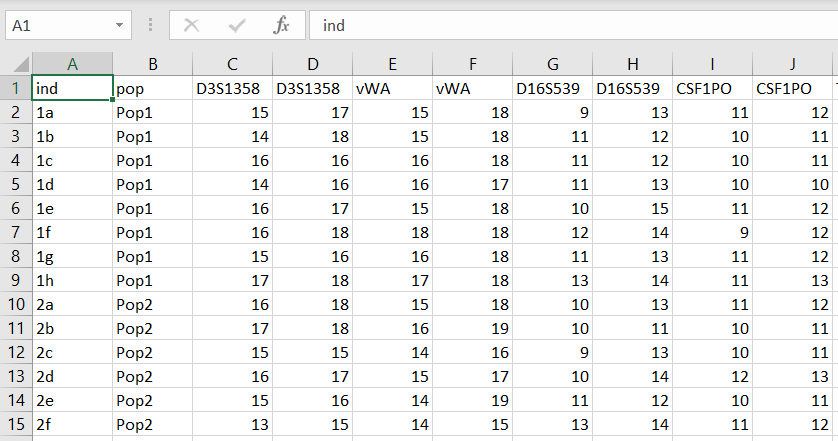
\includegraphics[width=1\linewidth]{img/capture_excel_1}

Then, one simply needs to save this table as a tab-delimited text file. This can be
achieved by clicking on \texttt{Save\ As} \textgreater{} \texttt{Text\ (Tab-delimited)\ (*.txt)}

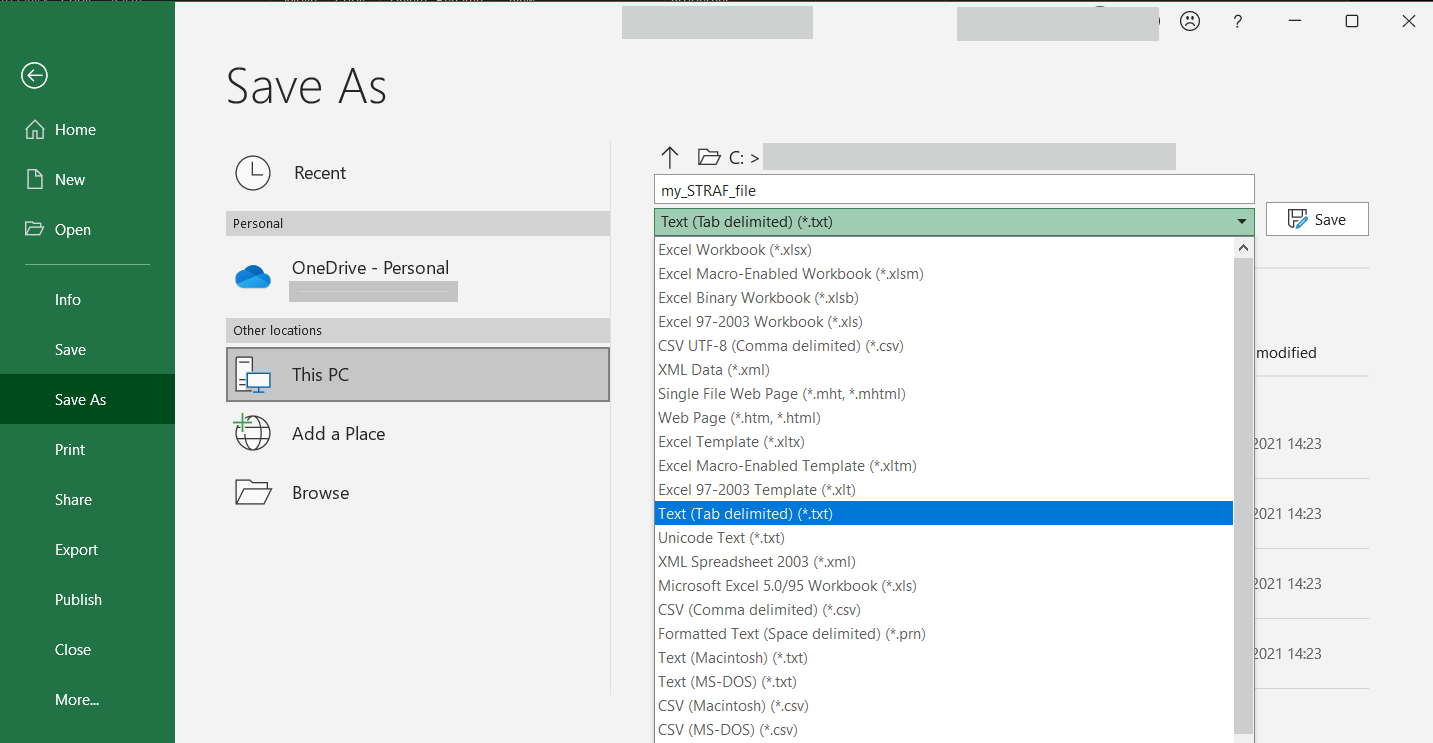
\includegraphics[width=1\linewidth]{img/capture_excel_2}

\hypertarget{uploading-the-data-to-straf}{%
\section{Uploading the data to STRAF}\label{uploading-the-data-to-straf}}

Once the input file has been prepared, it is possible to upload it into STRAF. Alternatively,
you can \textbf{download an example file} by clicking on the link in the sidebar.

Then, you need to select the \textbf{ploidy} of your data (for example, \emph{Diploid} for
autosomal markers, and \emph{Haploid} for Y-chromosome markers). After that, you can
upload the file by clicking on \emph{Browse} and selecting the file on your computer.

Once the file is uploaded, a preview will be displayed on the right and all the
analyses will be available. If not, it is likely that an error has occurred. If the error
message is not explicit, you can refer to the \textbf{Input file checklist} below that
gathers common issues with the input file.

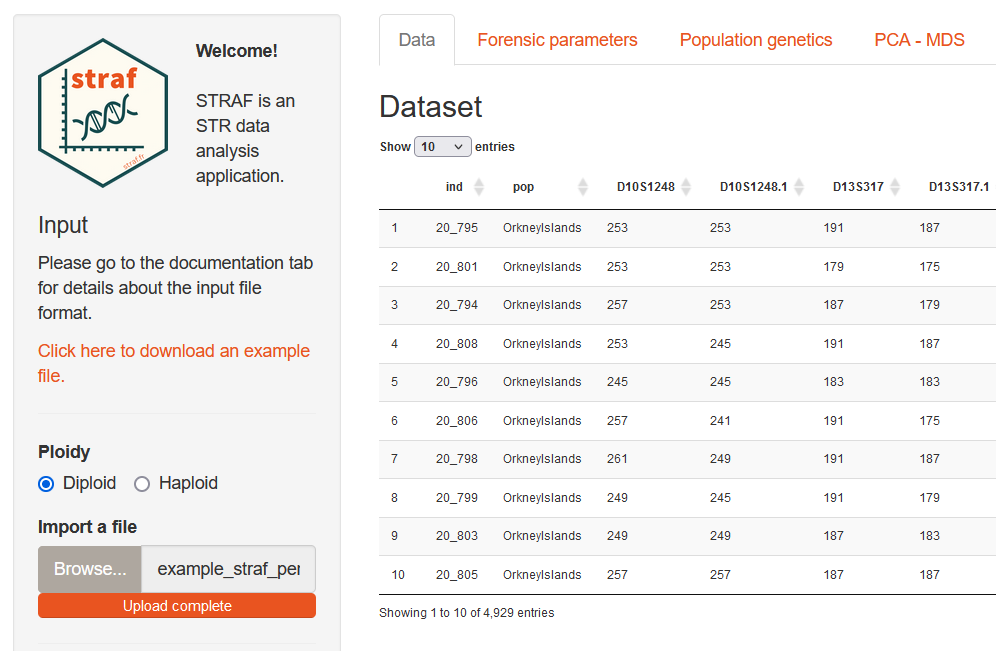
\includegraphics[width=1\linewidth]{img/capture_import_1}

\hypertarget{common-issues}{%
\section{Common issues}\label{common-issues}}

Even though you've been very careful in the generation of STRAF's input file,
it is possible that you still run into an error after uploading the file to STRAF.
In case STRAF cannot read your input file, we've put together a checklist to identify
common issues with the input file.

\begin{interpretation}

\textbf{Input file checklist}

\begin{itemize}
\tightlist
\item
  Check input parameters in the sidebar: do they actually correspond to the input data?
\item
  Check locus names: are they all different for haploid data? Do both columns for a single locus for diploid data have the exact same name?
\item
  Check that all missing data have been encoded with a ``0''
\item
  Try to remove any special characters from sample and locus names
\item
  Check for the presence of empty spaces at the end of each line
\item
  Check if alleles are exclusively encoded with numbers
\item
  Check if values are separated by tabs and not spaces
\item
  Check if the first two columns are names ``ind'' and ``pop''
\end{itemize}


\end{interpretation}

\hypertarget{having-a-first-look-at-the-data}{%
\section{Having a first look at the data}\label{having-a-first-look-at-the-data}}

Below the dataset preview, you will be able to generate a plot of allele frequencies
at each locus.

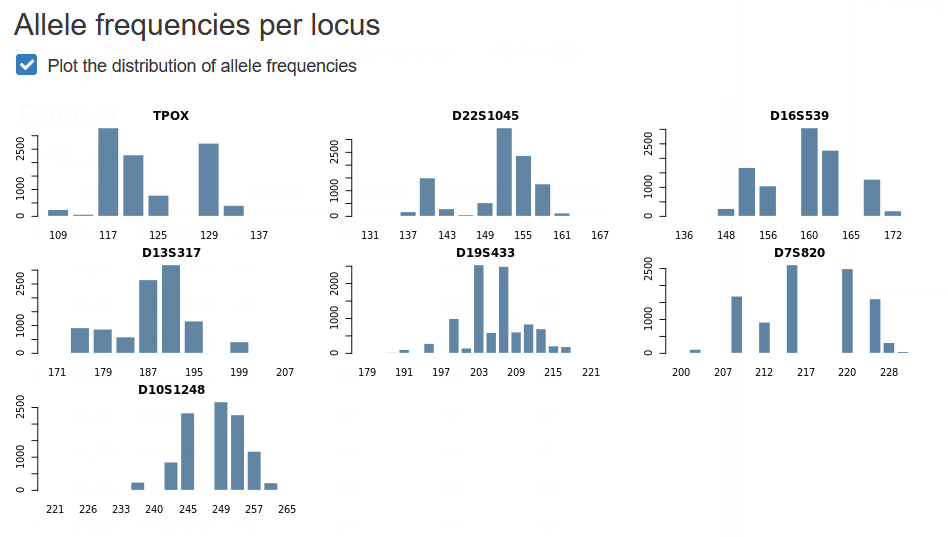
\includegraphics[width=1\linewidth]{img/capture_import_2}

You can also generate an allele frequency table, which is standard practice when
reporting new population data in a forensics journal. You can either download
the allele frequencies in a text format (TSV), or as an Excel (XLSX) file. Note
that you have the ability to select a specific population using the drop-down menu
above the table.

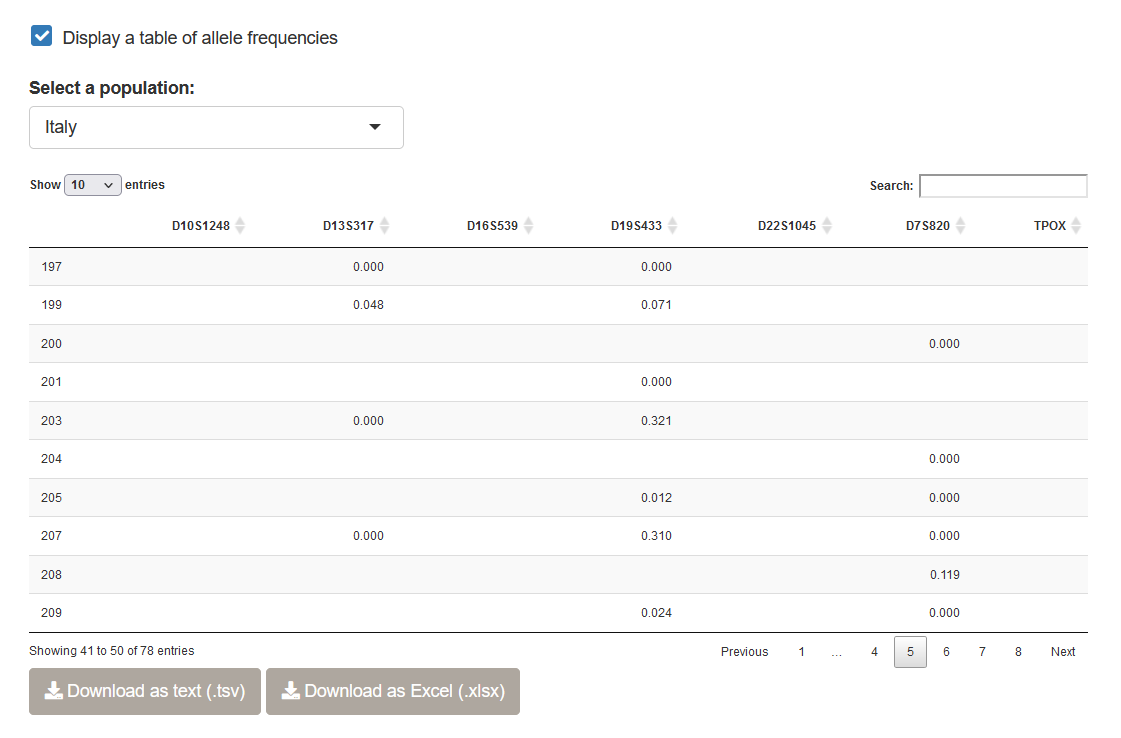
\includegraphics[width=1\linewidth]{img/capture_import_3}

\hypertarget{forensic-parameters}{%
\chapter{Forensic parameters}\label{forensic-parameters}}

In this chapter, we'll show how to compute forensic parameters using STRAF, and
provide details on how they are computed and should be interpreted.
We'll introduce a few equations, but please do not be afraid! The goal of
this chapter is to translate each of them into plain English.

\hypertarget{how-to-compute-forensic-parameters-in-straf}{%
\section{How to compute forensic parameters in STRAF}\label{how-to-compute-forensic-parameters-in-straf}}

Once your data has been uploaded, you can go to the \textbf{Forensic parameters} tab
and check the \emph{Compute forensics statistics} box. The computation will be performed
and a table containing the values per locus will be displayed. The computation is done
per population and overall, a drop-down menu is present to select the population.

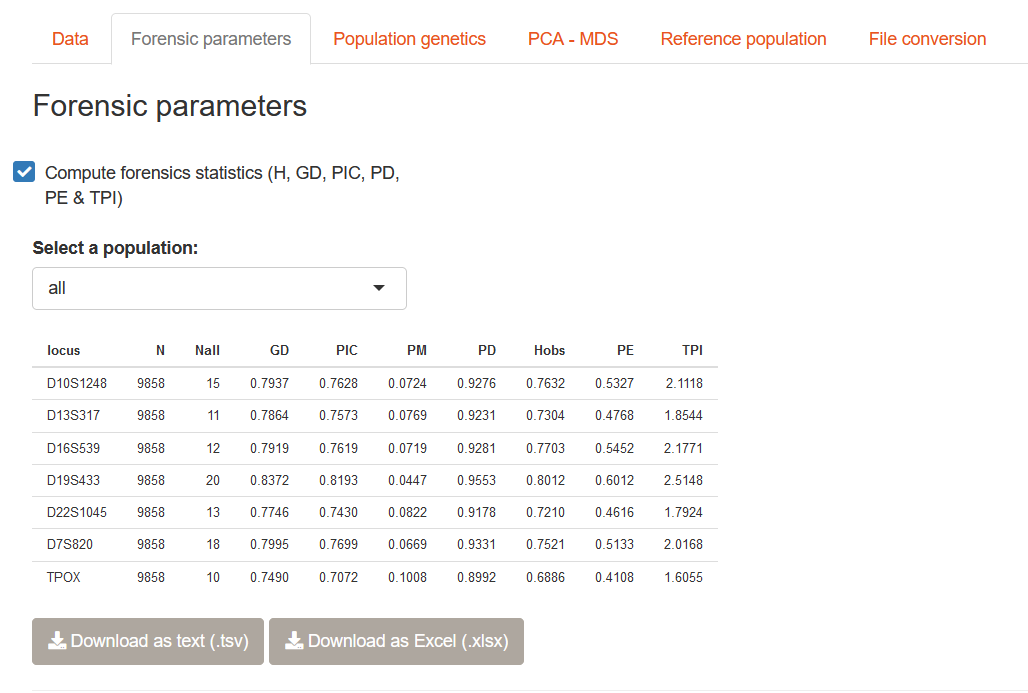
\includegraphics[width=1\linewidth]{img/capture_forensics_parameters_1}

Below the forensic parameters table, You can select the metric you would like
to represent using the drop-down menu.

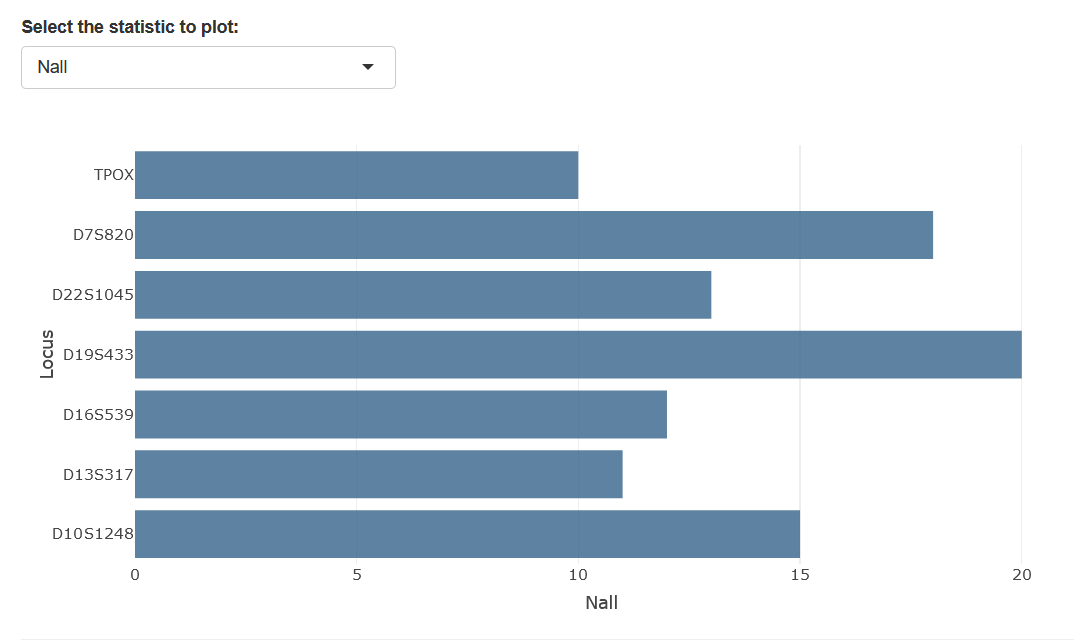
\includegraphics[width=1\linewidth]{img/capture_forensics_parameters_2}

\hypertarget{details-on-the-forensic-parameters}{%
\section{Details on the forensic parameters}\label{details-on-the-forensic-parameters}}

\hypertarget{random-match-probability-pm}{%
\subsection{Random match probability (PM)}\label{random-match-probability-pm}}

The \textbf{Random match probability}, or probability of matching (PM), is defined as
the probability of observing a random match between two unrelated individuals.

\textbf{Formula}

\[
PM = \sum_i (G_i)^2,
\]
where \(G_i\) is the frequency of the genotype \(i\) at a given locus in the population.

\textbf{Interpretation}

Computing \(PM\) means calculating, for a given locus, the frequency of each
genotypes. Then we take the square of each frequency, i.e.~we multiply it by itself.
Finally, we sum the values of each genotype.

The intuition behind it is that if we observe a random match in a population when looking
at a single locus, it means that our two samples have the same genotype at that locus.
In terms of probabilities, sampling a specific genotype in the population has a probability
equal to its frequency. And sampling the same genotype a second time (i.e., observing a match),
is the probability of sampling this genotype multiplied by itself.

As an example, say the genotype ``12-14'' has a frequency of 5\% in the population, the probability of
having a random match between two individuals having the same genotype is 0.05 x 0.05.

To get an overall probability of matching, we sum this over all possible genotypes
in our population.

\hypertarget{power-of-discrimination-pd}{%
\section{Power of Discrimination (PD)}\label{power-of-discrimination-pd}}

The power of discrimination (PD) is defined as the probability of
discriminating between two unrelated individuals.

\textbf{Formula}

\[
PD = 1 - PM
\]

\textbf{Interpretation}

PD is simply 1 - PM. Instead of looking at the probability of matching, we are
interested in the probability of ``not matching'', i.e.~the probability of discrimination.

\hypertarget{gene-diversity}{%
\section{Gene diversity}\label{gene-diversity}}

\textbf{Gene diversity} (\(GD\), sometimes simply \(D\)), also called \textbf{expected heterozygosity}
(\(H_{\mathrm{exp}}\)), is computed using the following estimator:

\textbf{Formula}

\[
  H_{\mathrm{exp}} = GD = \frac{n}{n - 1} \left( 1 - \sum_{i=1}^{n}(p_i)^2 \right),
\]

where \(n\) is the number of gene copies sampled (i.e., the sample size for haploid samples, and twice the sample size for diploid samples) and \(p_i\) is the
frequency of the \(i^{th}\) allele in the population.

\textbf{Interpretation}

It is the probability that an individual will be heterozygous at a given locus.

As an example, a value of \(GD\) of 0.6 means that there is a 60\% chance of being
heterozygote at this locus.

It depends directly on the genetic diversity at this locus, which itself depends on
allele frequencies in your population.

Say we have two alleles in a given population, genetic diversity will be higher
in a population with allele frequencies 0.5 and 0.5 than in a population where
frequencies are 0.1 and 0.9 (as less heterozygotes can be made with rare
alleles). This rationale can be extended to any number of alleles.

\hypertarget{polymorphism-information-content-pic}{%
\section{Polymorphism Information Content (PIC)}\label{polymorphism-information-content-pic}}

\textbf{Formula}

The \textbf{Polymorphism Information Content} (PIC) is computed as follow:

\[
PIC = 1 - \sum_{i=1}^{n} p_i^2 - \sum_{i=1}^{n-1} \sum_{j=i+1}^{n} 2p_i^2p_j^2,
\]
where \(p_i\) and \(p_j\) are allele frequencies.

\textbf{Interpretation}

The PIC can be interpreted as:

\begin{itemize}
\item
  the probability that the maternal and paternal alleles of a child are
  deducible
\item
  or, the probability of being able to deduce which allele a
  parent has transmitted to the child.
\end{itemize}

\hypertarget{power-of-exclusion-pe}{%
\section{Power of Exclusion (PE)}\label{power-of-exclusion-pe}}

\textbf{Formula}

The \textbf{power of exclusion} (\(PE\)) is defined as:

\[
PE = h^2\left(1 - 2hH^2\right),
\]

where \(h\) is the proportion of heterozygous individuals and \(H\) the
proportion of homozygous individuals in the population sample.

\textbf{Interpretation}

The power of exclusion depends on the observed proportions of heterozygous and homozygous individuals in a population. These proportions, multiplied as in the equation above, give the \textbf{mean exclusion probability for a paternity test}. Intuitively, the more diverse the population is, the greater this value is, as diversity is related to heterozygosity (see above).

\hypertarget{typical-paternity-index-tpi}{%
\section{Typical Paternity Index (TPI)}\label{typical-paternity-index-tpi}}

Finally, the typical paternity index (\(TPI\)) reflects the ``mean PI for
random non-excluded men`` in trio cases (father-mother-child) for a given locus.

\textbf{Formula}

Let \(H\) be the frequency of homozygotes, then

\[
TPI = \frac{1}{2H}
\]

\textbf{Interpretation}

Unlike the other parameters, the typical paternity index values are not in the 0-1
range and cannot be interpreted as a probability. It is a ratio of 1 divided by
twice the frequency of homozygotes in the population. This is an \textbf{odds ratio},
measuring how many times more likely that a possible father is the actual
father than a randomly selected man in the population, on average (\emph{typical} case).

\hypertarget{popgen-indices}{%
\chapter{Population genetics indices}\label{popgen-indices}}

In this chapter, we will see how to compute some population genetics indices in STRAF.

\hypertarget{computing-population-genetics-parameters-in-straf}{%
\section{Computing population genetics parameters in STRAF}\label{computing-population-genetics-parameters-in-straf}}

Once you have uploaded your genotypes in STRAF, you can go to the \textbf{Population genetics}
tab to compute relevant population genetics indices. It is also possible to perform
a Hardy-Weinberg equilibrium test by checking the relevant box.

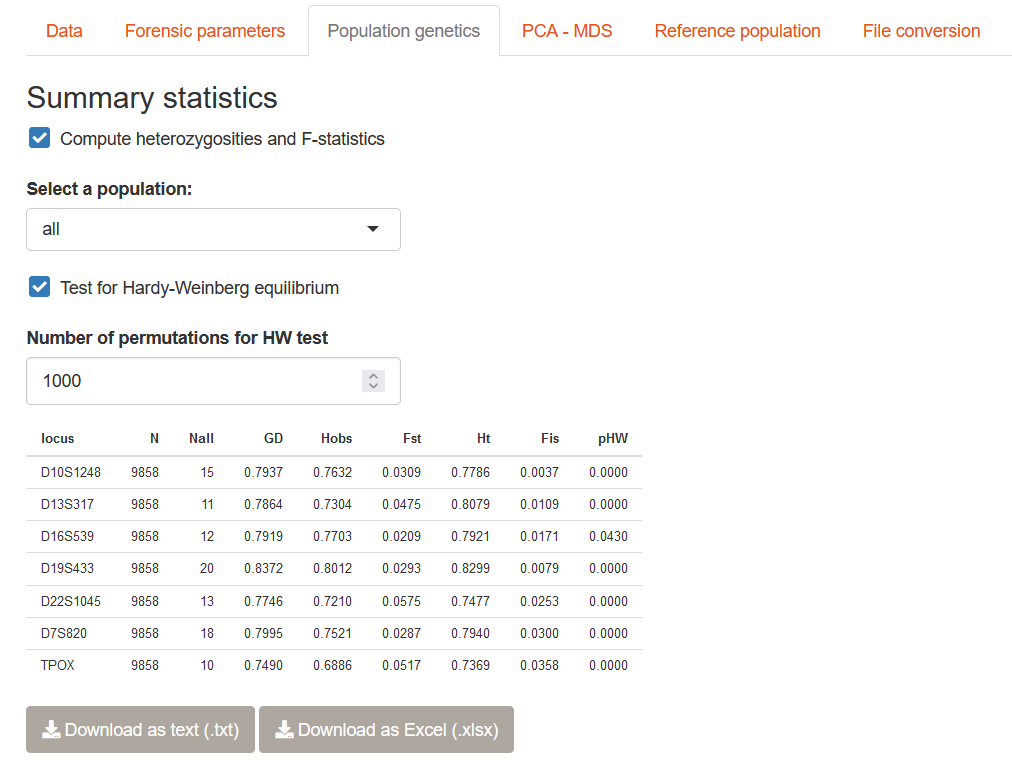
\includegraphics[width=1\linewidth]{img/capture_popgen_parameters_1}

\hypertarget{details-on-population-genetics-indices}{%
\section{Details on population genetics indices}\label{details-on-population-genetics-indices}}

\hypertarget{hardy-weinberg-equilibrium}{%
\subsection{Hardy-Weinberg equilibrium}\label{hardy-weinberg-equilibrium}}

A population is considered at Hardy-Weinberg equilibrium (HWE) when the observed
genotypic frequencies are in agreement with the expectations in an ``ideal'' population,
which assumes for example random mating in the population.
This is important as the assumptions of the Hardy-Weinberg model
allow to derive quantities such as forensic parameters and population genetic indices.
Therefore, if some assumptions of the model are violated, conclusions drawn from
metrics computed assuming HWE could be challenged.

If a locus presents a significant deviation from HWE, it means that a process
is influencing the distribution of allele and genotype frequencies in the population.
It could for example be due to \textbf{inbreeding}, \textbf{hidden population structure},
or \textbf{natural selection}.

STRAF reports the \textbf{p-value} of a test for HWE. A low p-value indicates a significant
deviation from HWE.

\hypertarget{heterozygosities}{%
\subsection{Heterozygosities}\label{heterozygosities}}

In STRAF, several measures of \textbf{heterozygosity} are computed. They capture
different aspects of genetic diversity.

\begin{itemize}
\item
  The \textbf{expected heterozygosity} (or \textbf{Gene diversity}, \(H_{exp}\) or \(GD\)) has been defined in the previous chapter.
\item
  The \textbf{observed heterozygosity} (\(H_{obs}\)) is the proportion of heterozygous genotypes at this locus in the population.
\item
  The \textbf{total heterozygosity} (\(H_T\)) is the heterozygosity expected if all the
  individuals in all the subpopulations were behaving as a population at HWE.
\end{itemize}

\hypertarget{f-statistics}{%
\subsection{F-statistics}\label{f-statistics}}

STRAF reports two \textbf{F-statistics}.

\begin{itemize}
\item
  The \(F_{\textrm{IS}}\) is a measure of genetic relatedness within a population.
  It is sometimes called the \textbf{inbreeding coefficient}. High values indicate
  a high degree of inbreeding.
\item
  The \(F_{\textrm{ST}}\) is a measure of genetic differentiation between populations.
  It takes values between 0 (no differentiation) and 1 (full differentiation).
\end{itemize}

\begin{interpretation}
\textbf{One concept, multiple estimators.}

Several \textbf{estimators} of \(F_{\textrm{ST}}\) exist (for example, Weir and Cockerham's, Nei's,
Hudson's \(F_{\textrm{ST}}\)). It's like if each population geneticist had decided
to develop their own estimator!

Why is that? In statistics, what we call an \textbf{estimator} is a metric aiming at estimating
a given quantity based on \textbf{observed data}. It is important to keep in mind that
these estimators rely on a specific \textbf{model}, with underlying assumptions.
It explains why some estimators are more or less reliable depending on the case
and observed data, and each of them has been developed for a different situation.
In the case of \(F_{\textrm{ST}}\) for example, different estimators assume
different demographic models.

\end{interpretation}

\hypertarget{linkage-disequilibrium-ld}{%
\section{Linkage disequilibrium (LD)}\label{linkage-disequilibrium-ld}}

\hypertarget{what-is-linkage-disequilibrium}{%
\subsection{What is linkage disequilibrium?}\label{what-is-linkage-disequilibrium}}

Linkage disequilibrium is an important quantity to be measured in genetics.
It is defined as the \textbf{nonindependence of genotypes at distinct loci}.
It means that it is more likely to observe the co-occurrence of some genotypes
at different loci. This can be influenced by population history.

However, most of the times, LD is explained by the physical proximity between loci. If
two loci are next to each other on the genome, recombination events between them
will be rare and genotypes won't be shuffled. Genotypes at these loci will be correlated
and linkage disequilibrium will be high. On the other hand, two loci found on two different
chromosomes are not expected to show any LD signals as genotypes will be systematically
shuffled at each generation.

\hypertarget{how-to-compute-ld-in-straf}{%
\subsection{How to compute LD in STRAF?}\label{how-to-compute-ld-in-straf}}

It is possible to test for the presence of LD in the dataset you uploaded using
STRAF. After checking the \emph{Display pairwise LD p-values matrix}, LD tests between
each pair of loci will be performed and p-values will be reported.

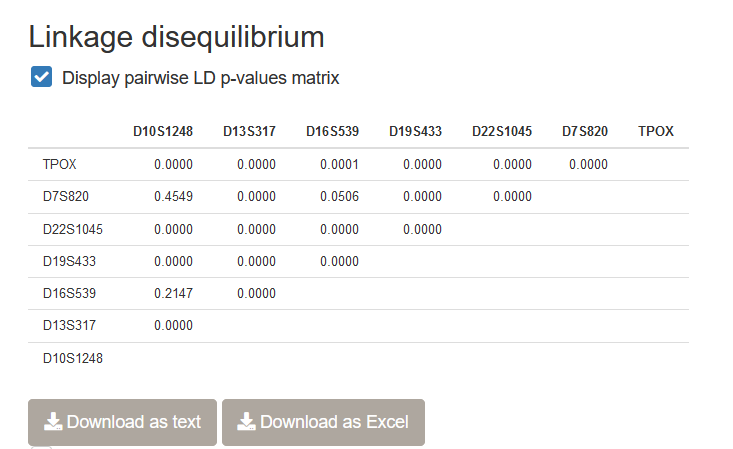
\includegraphics[width=1\linewidth]{img/capture_popgen_parameters_2}

\textbf{Important note}: Other population genetics software,
\textbf{Genepop} and \textbf{Arlequin}, implement more reliable
versions of the LD test that should be preferred. They are currently not implemented
in STRAF because of performance limitations. If you need to perform such a test, the
\textbf{File conversion} utilities (cf.~Chapter 6) should facilitate the workflow.

\hypertarget{pca-mds}{%
\chapter{Multivariate statistics}\label{pca-mds}}

In this chapter, we will describe the two multivariate statistics methods implemented
in STRAF, \textbf{Principal Component Analysis} (\textbf{PCA}) and \textbf{Multidimensional Scaling} (\textbf{MDS}).

\hypertarget{principal-component-analysis-pca}{%
\section{Principal Component Analysis (PCA)}\label{principal-component-analysis-pca}}

PCA is a method of \textbf{dimensionality reduction}. What is does it that it tries to
\textbf{capture most of the variation} present in the data and \textbf{project} it onto a
small number of new axes called \textbf{principal components} (PCs).

This is a useful method to capture variation from a large number of variables and
allows to discover hidden patterns by increasing interpretability.

In our case, if we consider that \textbf{each allele at each locus} is a variable, and that
our individual observations are the presence / absence of each allele for each sample,
we end up with a highly dimensional dataset (we have as many variables as we have
alleles!). It gets even worse if you analyse genome sequences, where you can have millions
of variables in your dataset. This is definitely not an interpretable dataset if you
are not able to easily extract relevant information.

PCA allows to bring most of the variation existing between our samples onto a few
axes capturing most of the variation (PCs).

In STRAF, you can perform a PCA by going into the \textbf{PCA - MDS} tab and checking
the following \emph{Run and plot a PCA} checkbox.

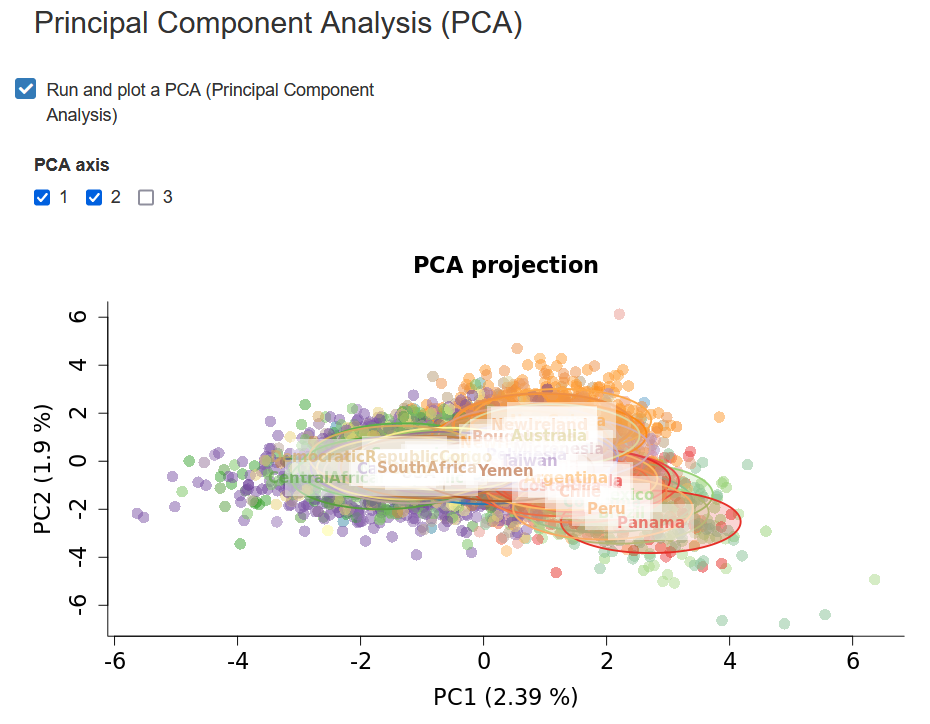
\includegraphics[width=1\linewidth]{img/capture_pca_1}

It will trigger the PCA computation and return a graph. You are also able to
download the coordinates of the samples on different PCs (also called eigenvectors).

\begin{interpretation}
\textbf{Interpreting PCA results}

PCA has become a popular tool in population genetics, as the relationships between
individuals on the PCA projection tend to reflect their genetic \textbf{relatedness}. The
closer individuals are on the PCA projection, the more genetically related they tend to be.

It can also be used as a \textbf{quality control} tool. For example, if a sample is very far
from all the others, including the ones that are part of the same population,
it is possible that there is an issue with the data. One would need to inspect
the raw data and check if any strange pattern can be found.

It is important to be aware of the influence of non-demographic processes on
the PCA projection. For example, \textbf{imbalanced sample sizes} between populations
can drive some patterns. When populations are sampled unevenly, the projection will
be \textbf{distorted} and distances observed on the projection can be driven by these
differences and not by their evolutionary history.

Hence, as multiple processes influence the results, PCA should remain an
\textbf{exploratory approach} and further analyses should be conducted before drawing
any major conclusions on the relationships between populations and individuals.

\end{interpretation}

\hypertarget{multidimensional-scaling-mds}{%
\section{Multidimensional Scaling (MDS)}\label{multidimensional-scaling-mds}}

An \textbf{MDS} is conceptually similar to a PCA. One of the main differences is
that it requires input data to be in a different format. As PCA uses raw genotypes and
can accommodate data at the individual level, \textbf{pairwise distances} between data
points are used for an MDS.

In forensics, it is typically used to compare \textbf{populations} and not
\textbf{individuals}, even though it would be theoretically possible.

As \textbf{pairwise distances between populations} are used, and MDS can be based on
any genetic distance: one could for example compute pairwise \textbf{FSTs},
\textbf{Nei's genetic distance}, or any other metric.

Based on these distances, the MDS will \textbf{project} the populations onto a
\textbf{lower-dimensional space}. This projection facilitates the interpretation of
relationships between populations.

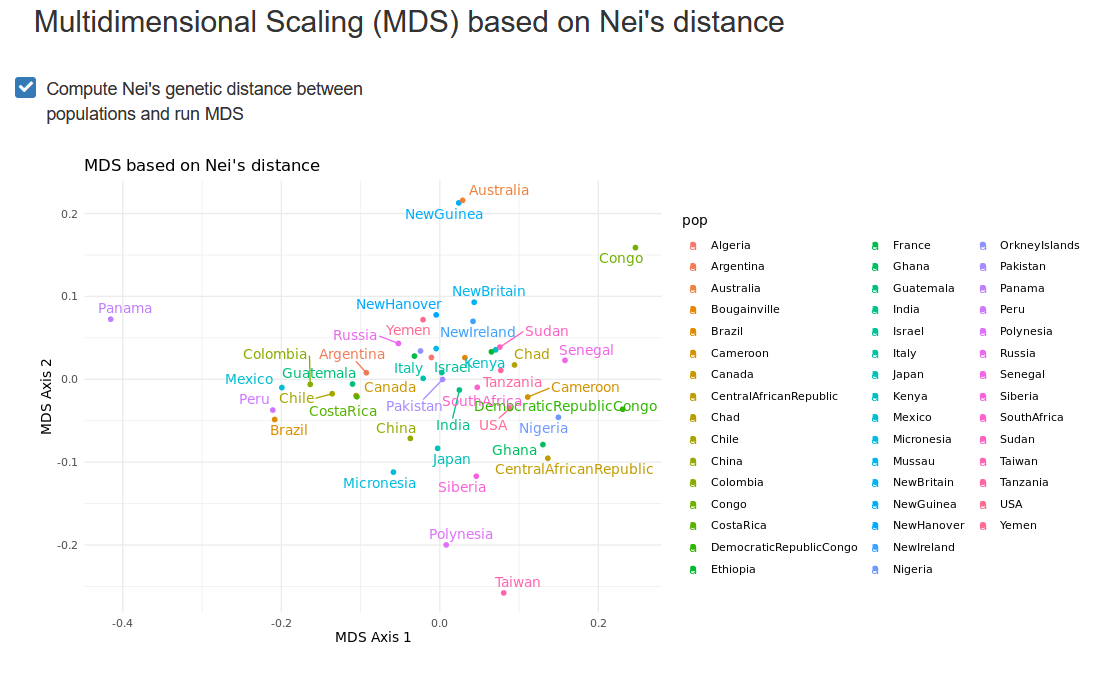
\includegraphics[width=1\linewidth]{img/capture_mds_1}

\begin{interpretation}
\textbf{Interpreting MDS results}

Just like with a PCA, the \textbf{closer} populations are on the MDS projection,
the more \textbf{genetically related} they tend to be, based on the markers that have been
used to compute their pairwise genetic distances.

Again, like for the PCA, the MDS should remain an
\textbf{exploratory approach} and further analyses should be conducted before drawing
any major conclusions on the relationships between populations and individuals.

\end{interpretation}

\hypertarget{ref-pop}{%
\chapter{Reference populations analysis}\label{ref-pop}}

In this chapter, we will see how to compare the uploaded populations to
reference populations (based on allele frequencies).

\hypertarget{mds-on-reference-frequencies}{%
\section{MDS on reference frequencies}\label{mds-on-reference-frequencies}}

STRAF implements an MDS computation based on allele frequency data. By default,
allele frequencies from the STRiDER database \citep{ref_strider} are used (loci with less than 10
populations have been excluded). If you are not familiar with the MDS method and
interpretation, you can find details in \textbf{Chapter 4}.

You can see the output of the MDS in the \textbf{Reference population} tab. It includes the
MDS projection in two dimensions for 19 European populations, as well as the population
tree.

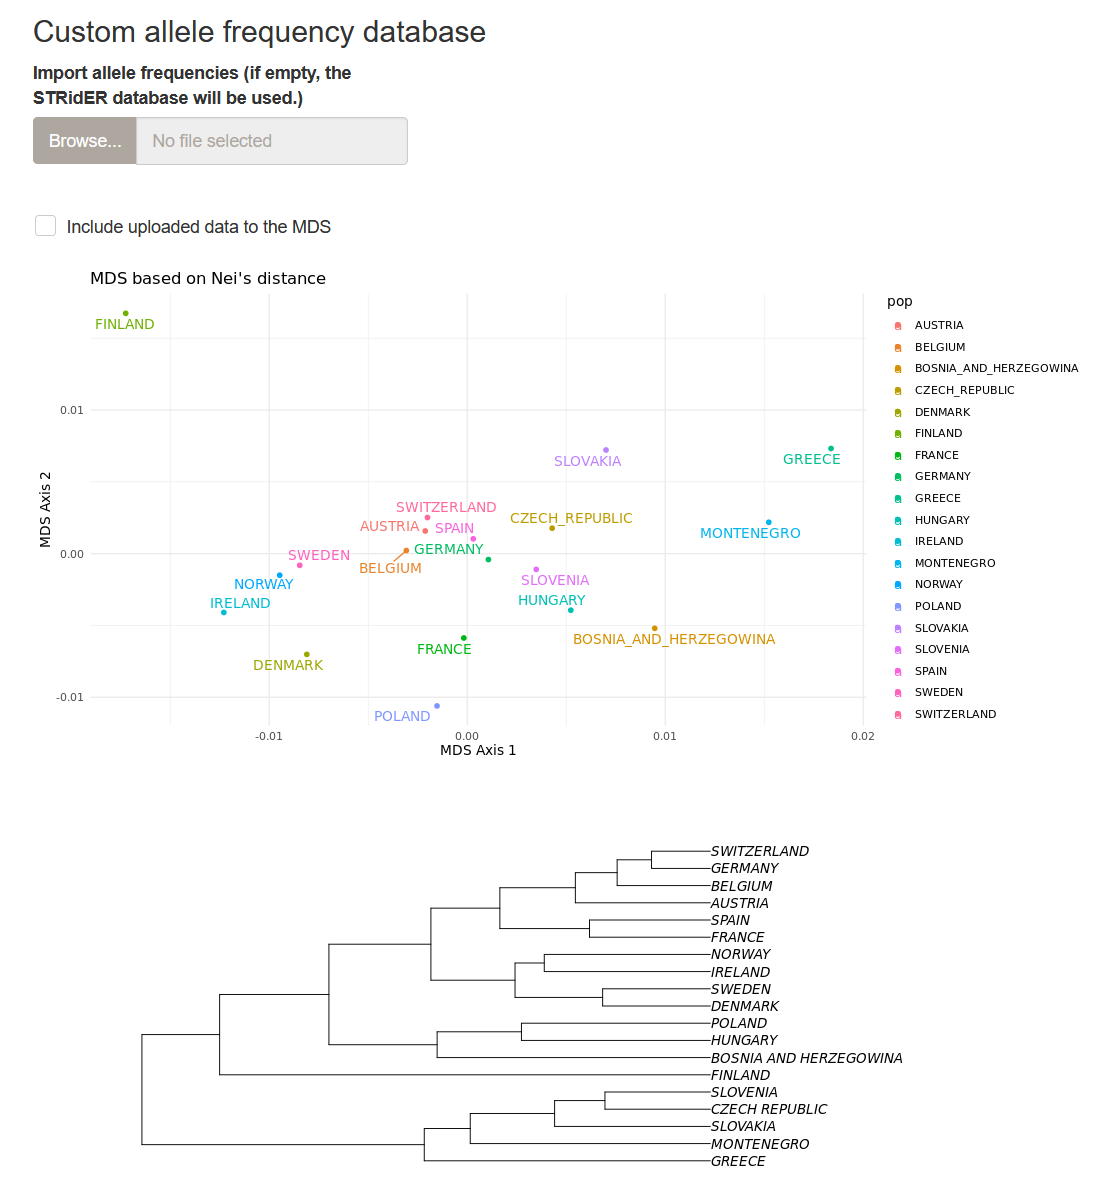
\includegraphics[width=1\linewidth]{img/capture_ref_pop_1}

The drop-down menu below the plots allows one to select or unselect populations
to be used in the MDS analysis.

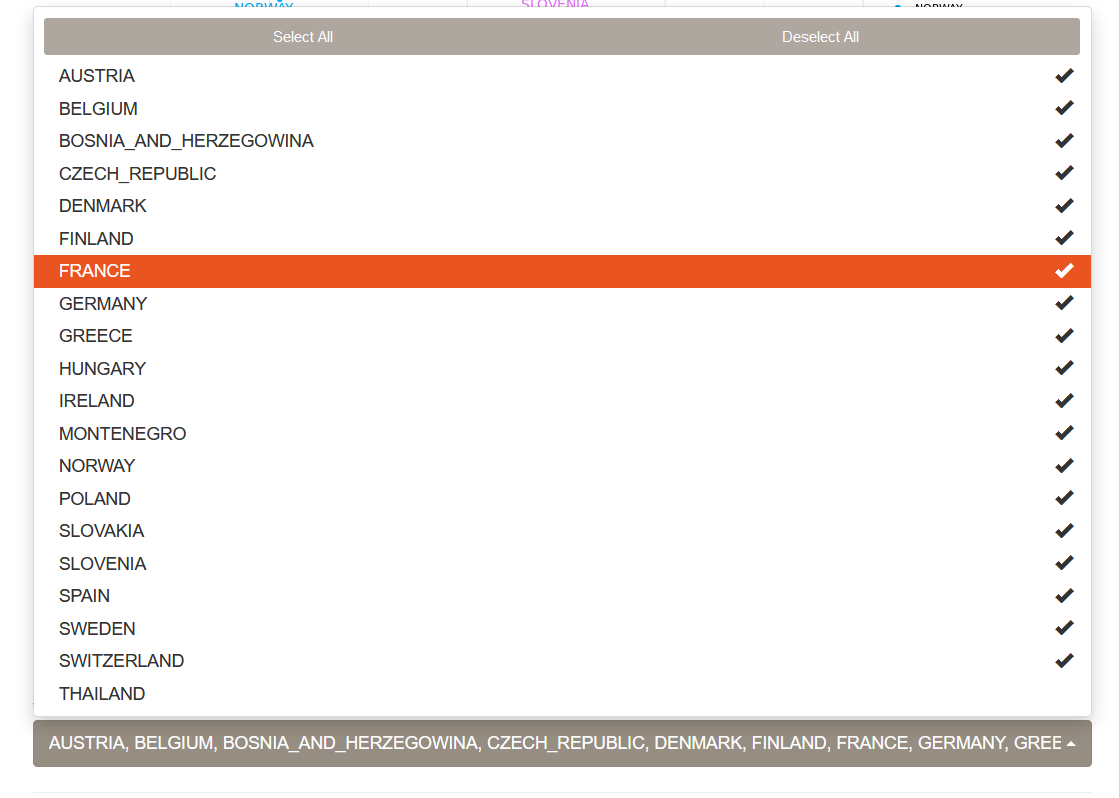
\includegraphics[width=1\linewidth]{img/capture_ref_pop_2}

Provided that some loci are in common between the reference allele frequencies and
the genotypes you uploaded, it is possible to add your own populations to the existing MDS
by checking the \emph{Include uploaded data to the MDS} box.

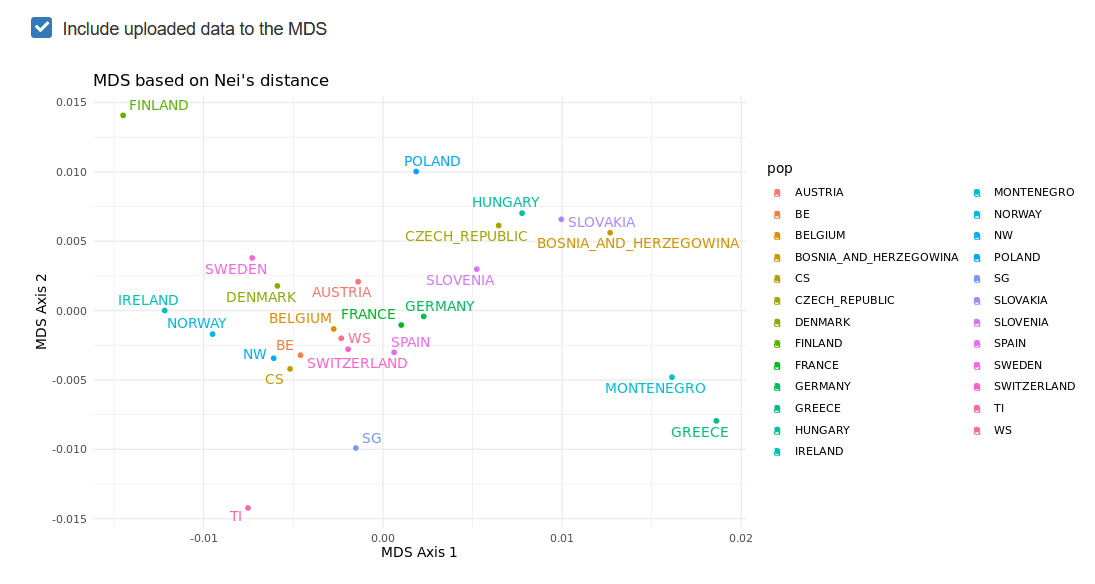
\includegraphics[width=1\linewidth]{img/capture_ref_pop_3}

You will then see your populations added to the MDS plots.

\hypertarget{preparing-a-custom-allele-frequency-database}{%
\section{Preparing a custom allele frequency database}\label{preparing-a-custom-allele-frequency-database}}

If you want to use other reference databases than STRIDER, for example if you're working with
non-European samples or with different loci, it is possible to upload a custom
allele frequency database in STRAF.

The data must be formatted as follows:

\begin{longtable}[]{@{}llll@{}}
\toprule
D1S1656 & & &\tabularnewline
\midrule
\endhead
Allele & Switzerland & Germany & France\tabularnewline
9 & 0.12 & 0.09 & 0\tabularnewline
10 & 0.40 & 0.35 & 0.28\tabularnewline
10.2 & 0.31 & 0.41 & 0.5\tabularnewline
11 & 0.17 & 0.15 & 0.22\tabularnewline
\textbf{D2S1338} & & &\tabularnewline
Allele & Switzerland & Germany & France\tabularnewline
19 & 0.40 & 0.38 & 0.42\tabularnewline
20 & 0.29 & 0.26 & 0.28\tabularnewline
21 & 0.31 & 0.36 & 0.3\tabularnewline
\bottomrule
\end{longtable}

Starting from an Excel file for example, we can start with a spreadsheet that looks
like this:

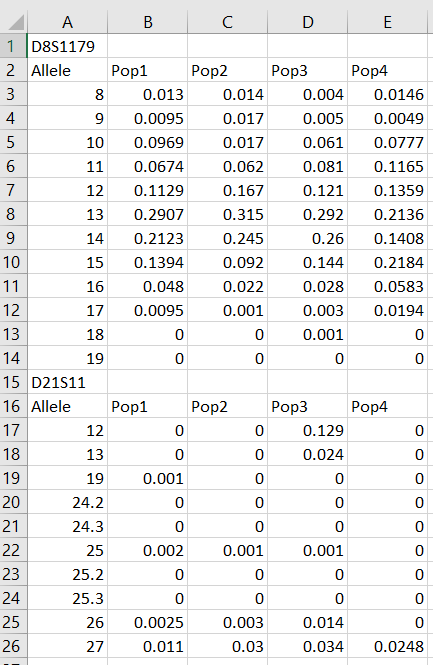
\includegraphics[width=1\linewidth]{img/capture_ref_excel_1}

Then, one simply needs to save this table as a CSV (Comma-Separated Values) file. This can be
achieved by clicking on \texttt{Save\ As} \textgreater{} \texttt{CSV\ (Comma-delimited)\ (*.csv)}.

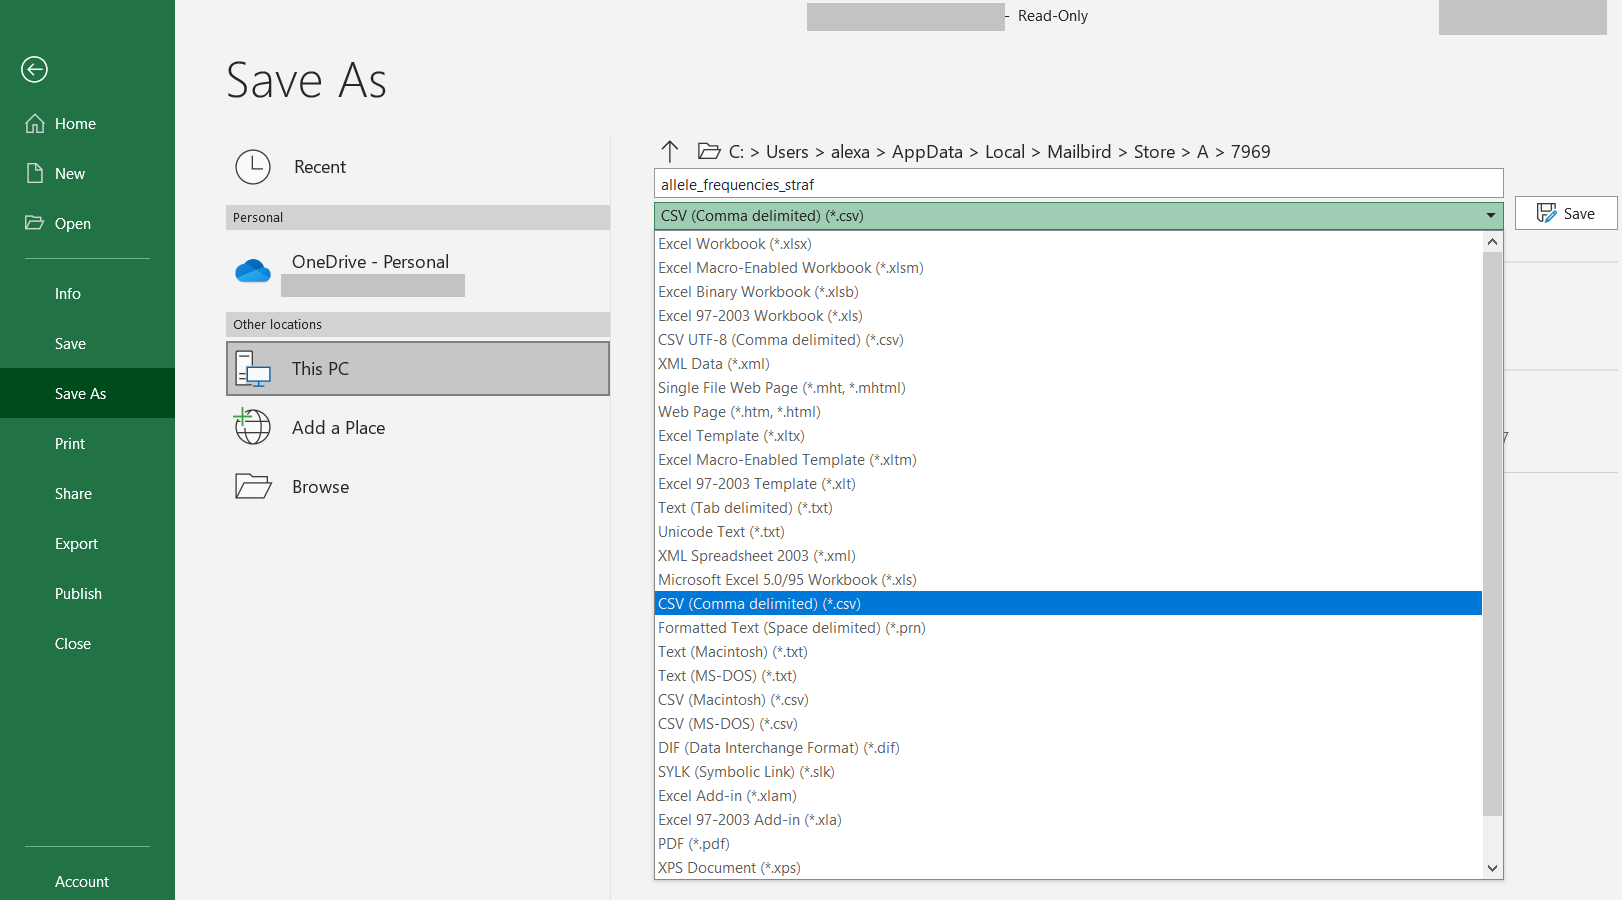
\includegraphics[width=1\linewidth]{img/capture_ref_excel_2}

Then, you can upload your data and use it as described for the STRIDER database.

\hypertarget{file-conversion}{%
\chapter{File conversion}\label{file-conversion}}

As STRAF is a web application and can be used simultaneously by multiple users,
computing resources are limited. Therefore, the most computationally intensive analyses
are not available in STRAF. In order to ease the path to other software,
file conversion utilities have been implemented. It is possible to convert
the input file to the \textbf{Genepop}, \textbf{Arlequin} and \textbf{Familias} formats. They are
all available in the \textbf{File conversion} tab of the application.

\hypertarget{how-to-convert-a-file-in-straf}{%
\section{How to convert a file in STRAF}\label{how-to-convert-a-file-in-straf}}

Once you have imported your file, it is straightforward to convert it to another
format. You can go to the \textbf{File conversion} tab and click on one of the following
buttons to download your genotypes in another format.

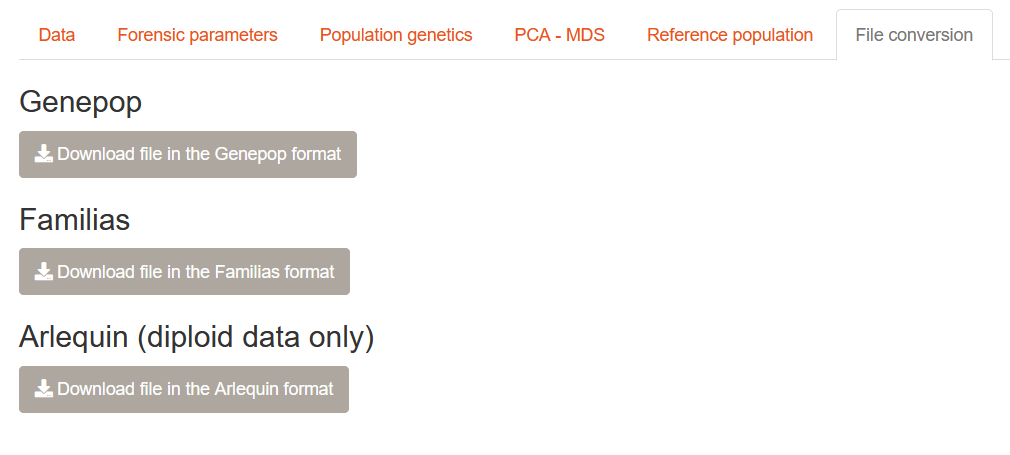
\includegraphics[width=1\linewidth]{img/capture_file_conversion_1}

\hypertarget{genepop-and-arlequin-formats}{%
\section{Genepop and Arlequin formats}\label{genepop-and-arlequin-formats}}

\textbf{Genepop} \citep{ref_genepop} and \textbf{Arlequin} \citep{ref_arlequin} softwares implement several population genetics methods,
including ones that are part of standard forensics practice:

\begin{itemize}
\item
  linkage disequilibrium computation
\item
  Hardy-Weinberg tests
\end{itemize}

STRAF currently implements these computations, however the ones implemented in
Genepop are overall more reliable as they can rely on more permutations. They
are overall preferable to the HW and LD tests implemented in STRAF.

\hypertarget{familias}{%
\section{Familias}\label{familias}}

Here a file containing allele frequencies is created. This file can be used in
Familias \citep{ref_familias} to provide allele frequency reference
data for relationship testing.

\hypertarget{snp-analysis}{%
\chapter{Analysing SNP data}\label{snp-analysis}}

\hypertarget{strs-vs.-snps}{%
\section{STRs vs.~SNPs}\label{strs-vs.-snps}}

STRs have been and remain the dominant marker used in forensic genetics.

This is mainly due to the fact that STRs have a high mutation rate, therefore
are more diverse in human populations. This explains their high \textbf{power of discrimination}.
Furthermore, they can also be used in deciphering mixture components, a very common
case in forensics. Finally, they can be combined in multiplex assays, which is convenient when lowamounts of biological material can be recovered.

Even though STRs will still remain the standard markers in forensic genetics
for many years, the application of sequencing data, especially the analyses
of SNPs became more and more popular in recent years.

Indeed, it nowadays easier and cheaper to generate whole-genome sequences than before.
One could wonder why STRs are still so popular in forensic practice, and have not been replaced by SNPs that are easily generated from Next-Generation Sequencing (NGS) data.

The advantages of SNPs are a higher multiplex capacity (with STRs and CE we can
analyse not much more than 25 markers in parallel) and therefore a higher
discriminative power and shorter amplicon size (interesting for degraded samples).

\hypertarget{how-to-analyse-snp-data-in-straf}{%
\section{How to analyse SNP data in STRAF?}\label{how-to-analyse-snp-data-in-straf}}

It is in theory possible to use any marker type in STRAF, as long as the input
format corresponds to what is expected from the software, that is:

\begin{itemize}
\item
  2 columns per locus for diploid data, 1 for haploid;
\item
  alleles are encoded by a number: for example, a diallelic SNP could be encoded as
  100 for the reference allele, and 101 for the alternative allele.
\end{itemize}

The main challenge remains encoding these values and converting from the initial
data format. As an example, a genotype table is easier to convert than raw sequences
or bioinformatics-specific formats such as the Variant Calling Format (VCF).

\hypertarget{conclusion}{%
\chapter{Conclusion}\label{conclusion}}

You have now reached the end of the STRAF Book. This book has been written to give
a broad overview of the concepts and tools you can find in the application.
We hope it has been useful to you.

If you want to know more about STRAF, you will find more information about the
software in the \textbf{Appendix} section.

You can now go back to \url{straf.fr} and use the application for your
forensics project! Any feedback is always welcome and you can contact us anytime.
STRAF is continuously improving thanks to your precious feedback!

\begin{figure}

\includegraphics[width=1\linewidth]{img/straf-logo} \caption{The STRAF logo.}\label{fig:straf-logo}
\end{figure}

\hypertarget{references}{%
\chapter{References}\label{references}}

\hypertarget{refs}{}

\hypertarget{acknowledgments}{%
\chapter{Acknowledgments}\label{acknowledgments}}

We thank STRAF's users for their useful comments and for giving the software
a reason to exist and be maintained. In particular, we would like to thank
Peter Vallone, Peter de Knijff, Guanglin He, Martin Bodner,
Nur Afiqah binti Hj Latip, Ritu Yadav, and Ömer Karataş.
We are grateful to them for sending their valuable feedback.

We are grateful to the University of Bern for covering the costs of STRAF hosting.

\hypertarget{appendix-appendix}{%
\appendix}


\hypertarget{technical-details}{%
\chapter{Technical details}\label{technical-details}}

\hypertarget{basic-information}{%
\section{Basic information}\label{basic-information}}

\begin{itemize}
\item
  STRAF is hosted on an Amazon Web Services (\textbf{AWS}) server located in \textbf{Ireland}.
\item
  STRAF has \textbf{2 CPUs} and \textbf{4 gigabytes of memory} available on the server. It is
  enough for the vast majority of cases, but might not be enough if your dataset
  is too large (too many samples, or too many loci).
\item
  The web application is based on the \textbf{R-Shiny framework}. \textbf{R} is an open source
  programming language particularly popular in data science. \href{https://www.rstudio.com/products/shiny/}{Shiny} is an
  open source \textbf{R} package that provides a web framework for building web
  applications using R.
\end{itemize}

\begin{figure}

\includegraphics[width=1\linewidth]{img/r-logo} \caption{The R logo.}\label{fig:r-logo}
\end{figure}

\hypertarget{understanding-strafs-performance}{%
\section{Understanding STRAF's performance}\label{understanding-strafs-performance}}

When you open STRAF, a new session. When you close your browser or the tab,
the session is closed and your data and computations are deleted.

STRAF can accept an unlimited number of user connections at the same time.
However, the computational resources are shared between users. In other words,
multiple users can connect at the same time, but computations will be ran one after
the other. If you wait longer than usual for a given task, it is likely
that someone else is using the server. Please keep this in mind and try to avoid
unnecessary computations!

STRAF has limited resources, as described above, and this can be limiting if your
dataset is too large because you have too many samples or loci. In that case,
you could consider trying to run STRAF locally as outlined in \textbf{Chapter} \ref{local-computer}. You could even host it on your own institution's server, in that
case feel free to contact us as we would be happy to help in the process.

\hypertarget{external-dependencies}{%
\section{External dependencies}\label{external-dependencies}}

STRAF wouldn't exist without the amazing community of R developers who contributed
great resources and packages.

The application uses several genetics packages:

\begin{itemize}
\item
  \texttt{genepop}
\item
  \texttt{edegenet}
\item
  \texttt{hierfstat}
\item
  \texttt{pegas}
\end{itemize}

More generic data science packages are also used:

\begin{itemize}
\item
  Shiny-related packages: \texttt{shiny}, \texttt{colourpicker}, \texttt{shinycssloaders}, \texttt{shinyWidgets}
\item
  The ``tidyverse'': \texttt{dplyr}, \texttt{tidyr}, \texttt{ggplot2}, \texttt{magrittr}, \texttt{openxlsx}, \texttt{reshape2}, \texttt{ggrepel}
\end{itemize}

\hypertarget{strafs-commitments}{%
\chapter{STRAF's commitments}\label{strafs-commitments}}

\hypertarget{straf-will-always-remain-free-and-open-source}{%
\section{STRAF will always remain free and open source}\label{straf-will-always-remain-free-and-open-source}}

STRAF is a \textbf{free} and \textbf{open-source} software. As free software advocates, we believe
anyone should be able to \textbf{run} the software, \textbf{study} the software,
\textbf{modify} the software, and to \textbf{share} copies of the software. That is why
STRAF is licensed under the permissive \textbf{GNU General Public License version 3}.
Here is the \href{https://www.gnu.org/licenses/gpl-3.0.txt}{full text of the GPL-3 license}.

For the most curious of you, you can view all the \href{https://github.com/agouy/straf}{source code of STRAF on GitHub}.

\hypertarget{straf-is-carbon-neutral}{%
\section{STRAF is carbon-neutral}\label{straf-is-carbon-neutral}}

Hosting a web application onto a server requires energy, and energy is becoming
more and more precious. For that reason, STRAF is hosted on a server that is
on a carbon-neutral data center and that will be fully powered by renewable energies by 2025.

This book and STRAF's code source are hosted onto GitHub servers, which are
carbon-neutral as well since 2019.

  \bibliography{references.bib}

\end{document}
